\chapter{Introduction}

Music is an essential part of human culture, history, and society. It has existed since ancient times and evolved, reflecting changes in our cultures, traditions, and beliefs. Despite its importance, the study of music has always been a challenging and complex task due to its subjective nature and the vast array of musical styles, genres, and cultures that exist worldwide.

Humanity has been studying music to understand its underlying structure for millennia. From the ancient Greeks, who believed that music had a mathematical and cosmic harmony, to the early works of theorists such as Rameau, Fux, and Schenker, and more recent approaches such as generative theory and corpus studies, music has been a subject of fascination and inquiry. This rich music theory and analysis history provide a valuable foundation for guiding and evaluating MIR algorithms and models. 

We all humbly seek to unlock the secrets of music's complex and multifaceted nature.

Music Information Retrieval (MIR) is a research area that has emerged in the last decades as an interdisciplinary field combining engineering, musicology, and neuroscience. MIR aims to develop algorithms and techniques to automatically analyze, classify, and retrieve musical information from audio signals. In my opinion, MIR research has been traditionally focused on technical aspects, such as digital signal processing (DSP), machine learning, and pattern recognition, neglecting other relevant domains, such as perception, cognition, music theory, aural skills, and musicology.

The reason behind this is non-other but the high implementation complexity for such heuristics and abstract fields of study.

%%%%%%%%%%%%%%%%%%

\begin{figure}[!ht]
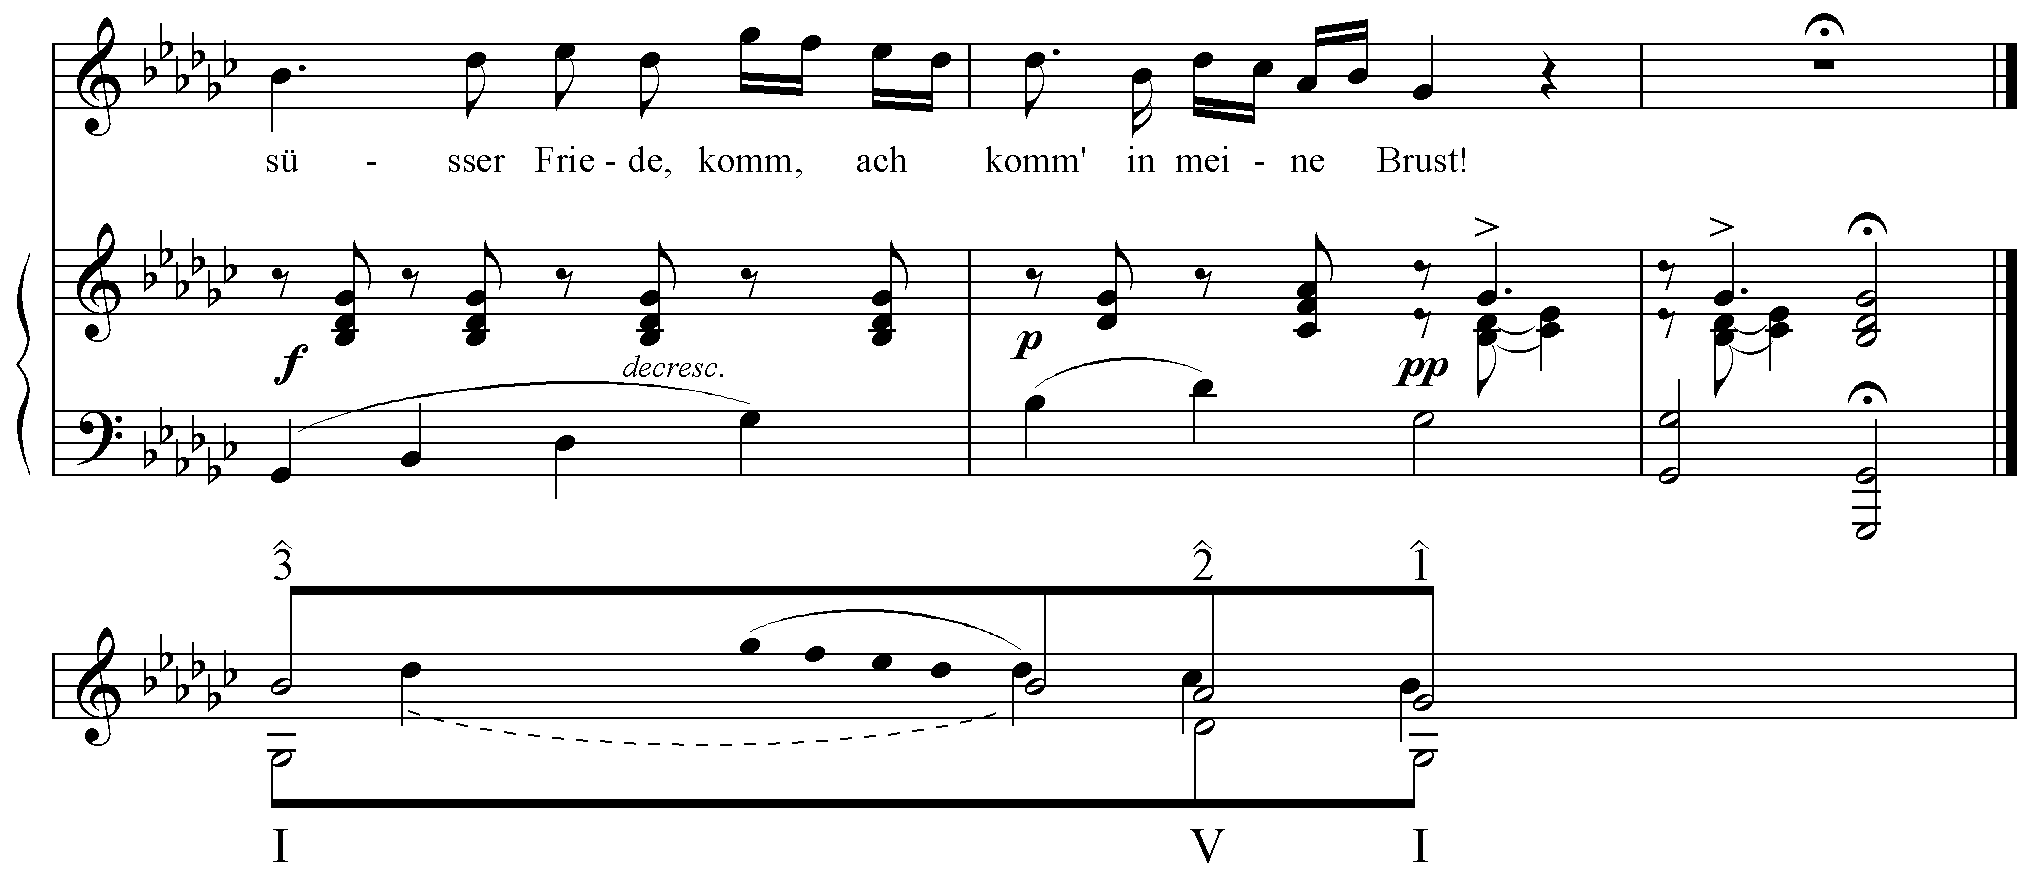
\includegraphics[clip,width=\columnwidth]{figures/schenkerian analysis/SchubertOp4no3.png}% 
\caption{Small excerpt of \textit{Wandrers Nachtlied, Op. 4, D. 224} by Franz Schubert. We can see the passage's original score, the schenkerian unfolding of the melody, the chord degrees, and the tonal function.}
\label{fig:timeseries}
\end{figure}

\begin{figure}[!ht]
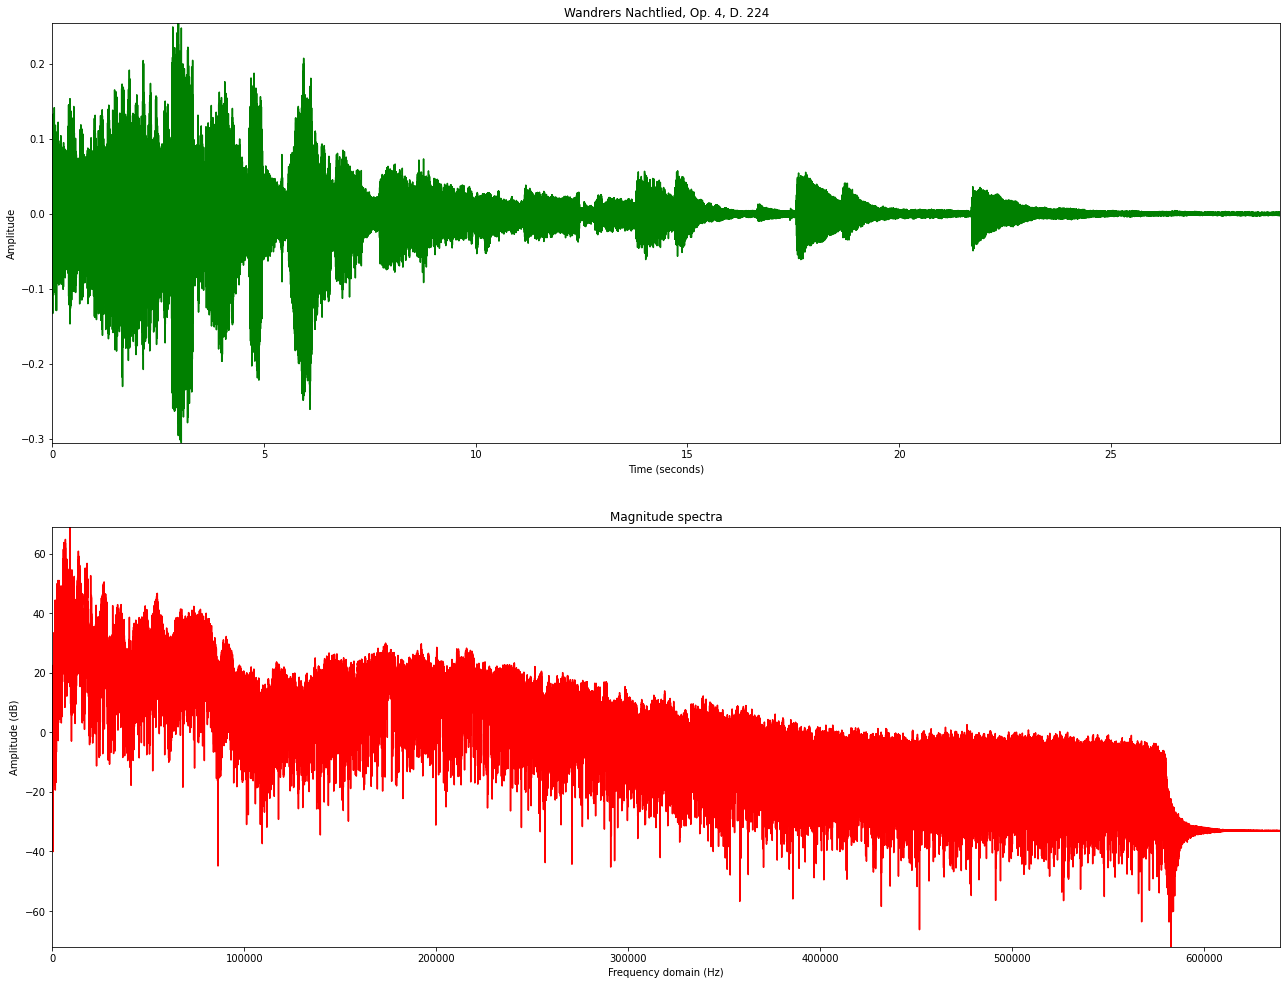
\includegraphics[clip,width=\columnwidth]{figures/schenkerian analysis/schubert.png}% 
\caption{\textit{Wandrers Nachtlied, Op. 4, D. 224} by Franz Schubert as performed by Dietrich Fischer-Dieskau and Jörg Demus}
\label{fig:timeseries}
\end{figure}

\begin{figure}[!ht]
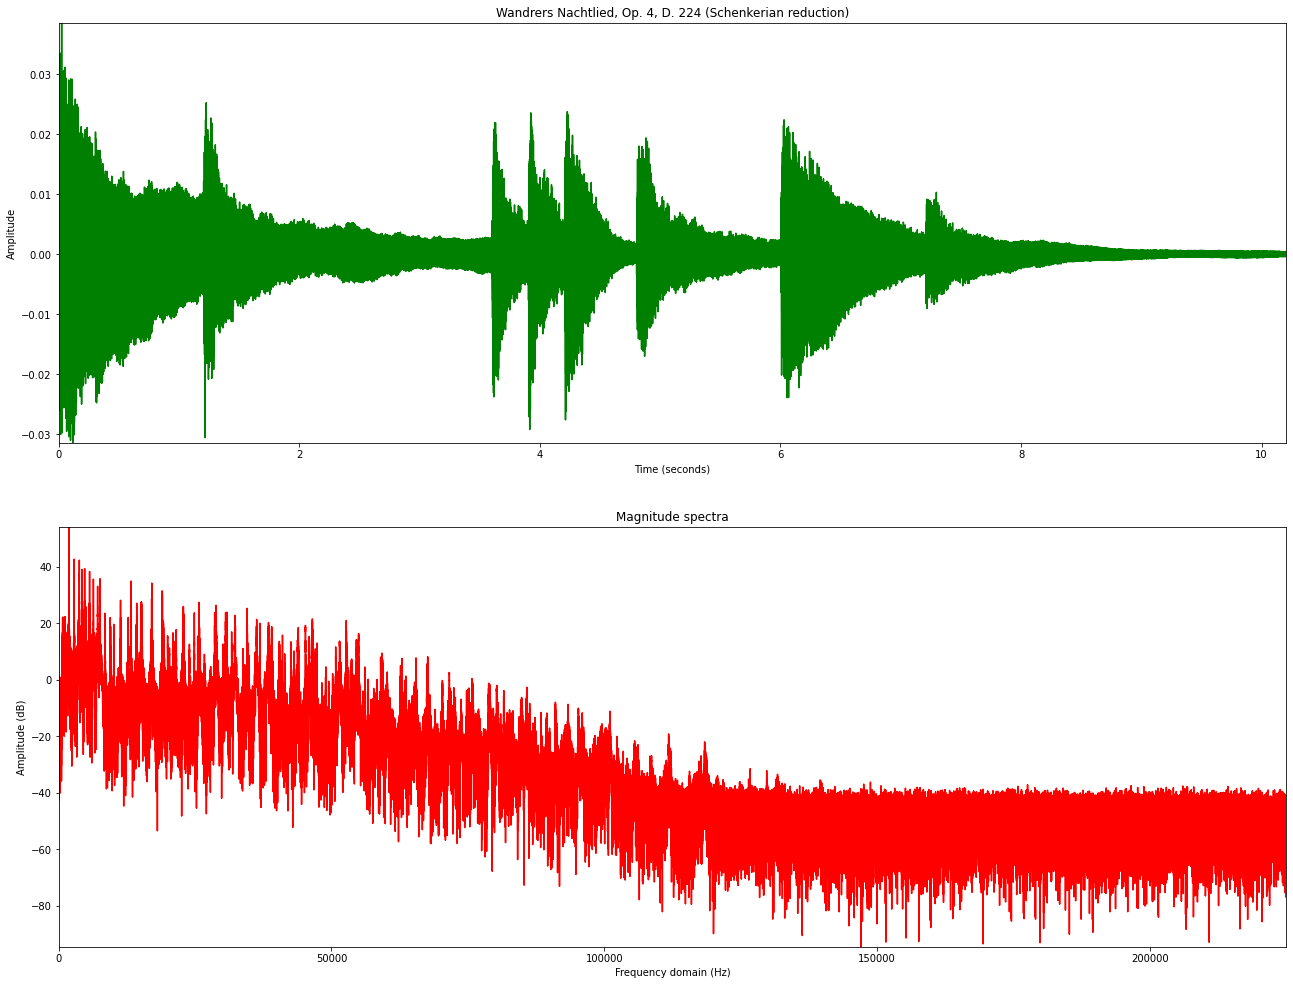
\includegraphics[clip,width=\columnwidth]{figures/schenkerian analysis/subert redu.png}% 
\caption{\textit{Wandrers Nachtlied, Op. 4, D. 224} by Franz Schubert (Schenkerian reduction or unfolding)}
\label{fig:timeseries}
\end{figure}

%%%%%%%%%%%%%%%%%%%%%%%%%%%%%%%%%%%%%%%%%%%%

\section{About aural skills and high-level perceptual}